\documentclass{standalone}
\usepackage{tikz}
\usetikzlibrary{calc}

\begin{document}
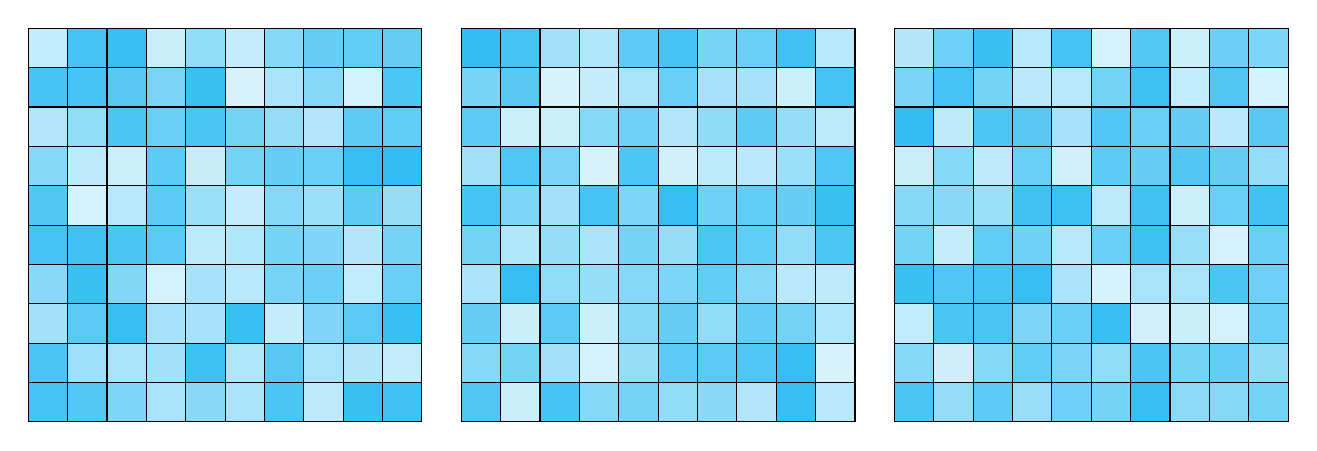
\begin{tikzpicture}
  % Draw a grid in green
  
  % Fill the diagonal with a gradient from green to blue
  \begin{scope}[scale=0.5]
  \foreach \a in {1,...,10}{
    \foreach \b in {1,...,10}{
      % Calculate a color that blends green and blue based on the position
      %% \pgfmathparse{}{int(\a*10)}
      %% \pgfmathsetmacro{\gridvalue}{\a*10}
      \pgfmathsetmacro{\gridvalue}{random(15,80)}
      \fill[cyan!\gridvalue!white] (\a-1,\b-1) rectangle (\a,\b);
      }
  }
  \draw[black] (0,0) grid (10,10);
  \end{scope}

  \begin{scope}[xshift=5.5cm,scale=0.5]
  \foreach \a in {1,...,10}{
    \foreach \b in {1,...,10}{
      % Calculate a color that blends green and blue based on the position
      %% \pgfmathparse{}{int(\a*10)}
      %% \pgfmathsetmacro{\gridvalue}{\a*10}
      \pgfmathsetmacro{\gridvalue}{random(15,80)}
      \fill[cyan!\gridvalue!white] (\a-1,\b-1) rectangle (\a,\b);
      }
  }
  \draw[black] (0,0) grid (10,10);
  \end{scope}

  
  \begin{scope}[xshift=11cm,scale=0.5]
  \foreach \a in {1,...,10}{
    \foreach \b in {1,...,10}{
      % Calculate a color that blends green and blue based on the position
      %% \pgfmathparse{}{int(\a*10)}
      %% \pgfmathsetmacro{\gridvalue}{\a*10}
      \pgfmathsetmacro{\gridvalue}{random(15,80)}
      \fill[cyan!\gridvalue!white] (\a-1,\b-1) rectangle (\a,\b);
      }
  }
  \draw[black] (0,0) grid (10,10);
  \end{scope}

\end{tikzpicture}
\end{document}
